% ============================================================
%  ArcDoc — PPGI/UnB Seminar — Updated Results
%  Compile: pdflatex seminar_arcdoc.tex  (2x)
%  Directory: CaVL-Doc/presentation/  (assets in ../docs/assets/)
% ============================================================
\documentclass[aspectratio=169,10pt]{beamer}

% ── Encoding ─────────────────────────────────────────────────
\usepackage[utf8]{inputenc}
\usepackage[T1]{fontenc}
\usepackage{lmodern}
\usepackage[english]{babel}

% ── Graphics and tables ──────────────────────────────────────
\usepackage{graphicx}
\usepackage{booktabs}
\usepackage{multirow}
\usepackage{colortbl}
\usepackage{xcolor}
\usepackage{array}
\usepackage{amsmath}
\usepackage{amssymb}
\usepackage{tikz}

\graphicspath{{../docs/assets/}}

% ── UnB colors ───────────────────────────────────────────────
\definecolor{unbblue}{HTML}{003875}
\definecolor{unbgreen}{HTML}{007B40}
\definecolor{unblight}{HTML}{E8F0F8}
\definecolor{coarserow}{HTML}{F5F5F5}
\definecolor{finerow}{HTML}{E3F2FD}
\definecolor{winrow}{HTML}{C8E6C9}

% ── Theme ────────────────────────────────────────────────────
\usetheme{Boadilla}
\usecolortheme[named=unbblue]{structure}

\setbeamercolor{title}{fg=white, bg=unbblue}
\setbeamercolor{subtitle}{fg=white!85, bg=unbblue}
\setbeamercolor{frametitle}{fg=white, bg=unbblue}
\setbeamercolor{block title}{fg=white, bg=unbblue}
\setbeamercolor{block body}{fg=black, bg=unblight}
\setbeamercolor{block title alerted}{fg=white, bg=unbgreen}
\setbeamercolor{block body alerted}{fg=black, bg=unblight}
\setbeamerfont{frametitle}{size=\normalsize, series=\bfseries}
\setbeamerfont{title}{size=\large, series=\bfseries}
\setbeamertemplate{navigation symbols}{}
\setbeamertemplate{itemize items}[circle]
\setbeamertemplate{enumerate items}[default]

% ── Logo embedded in the header bar ──────────────────────────
\logo{}
\setbeamertemplate{frametitle}{%
  \nointerlineskip
  \begin{beamercolorbox}[wd=\paperwidth, ht=2.4ex, dp=0.9ex,
                         leftskip=0.6em, rightskip=0.5em]{frametitle}%
    \usebeamerfont{frametitle}\insertframetitle\strut%
    \hfill%
    \raisebox{-0.25\height}{\includegraphics[height=0.42cm]{as_vert_cor.jpg}}%
  \end{beamercolorbox}%
}

% ── Macros ───────────────────────────────────────────────────
\newcolumntype{C}[1]{>{\centering\arraybackslash}p{#1}}
\newcolumntype{R}[1]{>{\raggedleft\arraybackslash}p{#1}}

% ── Metadata ─────────────────────────────────────────────────
\title[ArcDoc --- PPGI/UnB Seminar]{%
  ArcDoc: Angular Margin Optimization\\
  for Zero-Shot Document Classification}
\subtitle{Seminar --- Updated Results}
\author[J.\,P.\,Costa \textbar{} Li Weigang]{%
  \includegraphics[height=1.0cm]{as_comp_cor.jpg}\\[6pt]
  \textbf{Joao Paulo Costa}\\[3pt]
  {\small Advisor: Prof.\,Dr.\,\textbf{Li Weigang}}}
\institute[PPGI/CIC/UnB]{%
  Graduate Program in Informatics --- PPGI\\
  Department of Computer Science --- CIC\\
  University of Brasília --- UnB}
\date{August 2026}

\titlegraphic{}

% ============================================================
\begin{document}
% ============================================================

% ── SLIDE 1: TITLE ───────────────────────────────────────────
{
\setbeamertemplate{footline}{}   % no footer on the title slide
\begin{frame}[plain]
  \titlepage
\end{frame}
}

% ── SLIDE 2: MOTIVATION — VERIFICATION AT SCALE ──────────────
{
\logo{}
\begin{frame}{Motivation: Document Flow in a Branch Network}

\vspace{-6pt}

\begin{center}
\scalebox{1.08}{%
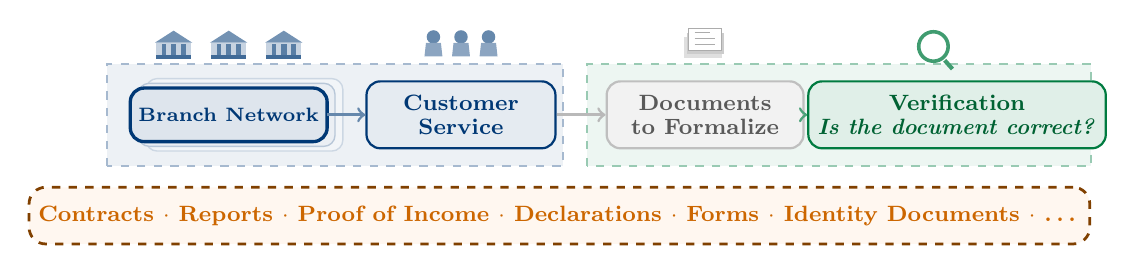
\begin{tikzpicture}

  % ══ ZONES ════════════════════════════════════════════════════
  \fill[unbblue!7]   (-0.3,-0.65) rectangle (5.5, 0.65);
  \draw[unbblue!35, dashed, line width=0.8pt] (-0.3,-0.65) rectangle (5.5, 0.65);
  \fill[unbgreen!7]  (5.8,-0.65) rectangle (12.2, 0.65);
  \draw[unbgreen!40, dashed, line width=0.8pt] (5.8,-0.65) rectangle (12.2, 0.65);

  % ══ VISUAL: BRANCH NETWORK (stacked boxes) ═══════════════════
  \fill[unbblue!5, rounded corners=4pt]  (0.20,-0.46) rectangle (2.70, 0.46);
  \draw[unbblue!20, line width=0.5pt, rounded corners=4pt] (0.20,-0.46) rectangle (2.70, 0.46);
  \fill[unbblue!8, rounded corners=4pt]  (0.10,-0.40) rectangle (2.60, 0.40);
  \draw[unbblue!28, line width=0.5pt, rounded corners=4pt] (0.10,-0.40) rectangle (2.60, 0.40);
  \fill[unbblue!13, rounded corners=5pt] (0.00,-0.34) rectangle (2.50, 0.34);
  \draw[unbblue, line width=1.2pt, rounded corners=5pt] (0.00,-0.34) rectangle (2.50, 0.34);
  \node[font=\scriptsize\bfseries, text=unbblue, text centered] at (1.25, 0.00)
    {Branch Network};

  % ══ MAIN NODES ════════════════════════════════════════════════
  \node[rounded corners=5pt, fill=unbblue!10, draw=unbblue, thick,
        minimum width=2.4cm, minimum height=0.85cm,
        text=unbblue, text centered, font=\footnotesize\bfseries] (atend) at (4.2, 0.0)
    {\shortstack{Customer \\ Service}};

  \node[rounded corners=5pt, fill=gray!10, draw=gray!50, thick,
        minimum width=2.5cm, minimum height=0.85cm,
        text=black!65, text centered, font=\footnotesize\bfseries] (docs) at (7.3, 0.0)
    {\shortstack{Documents \\ to Formalize}};

  \node[rounded corners=5pt, fill=unbgreen!12, draw=unbgreen, thick,
        minimum width=2.4cm, minimum height=0.85cm,
        text=unbgreen!80!black, text centered, font=\footnotesize\bfseries] (verif) at (10.5, 0.0)
    {\shortstack{Verification \\ \textit{Is the document correct?}}};

  % ══ ARROWS ════════════════════════════════════════════════════
  \draw[->, line width=1.0pt, color=unbblue!60] (2.50, 0) -- (atend.west);
  \draw[->, line width=1.0pt, color=gray!55]    (atend.east) -- (docs.west);
  \draw[->, line width=1.0pt, color=unbgreen!70] (docs.east) -- (verif.west);

  % ══ ICONS: 3 branches (network scale) ═════════════════════════
  \begin{scope}[shift={(0.55, 0.78)}, scale=0.85]
    \fill[unbblue!55] (-0.28,0.16) -- (0,0.34) -- (0.28,0.16) -- cycle;
    \fill[unbblue!22] (-0.26,-0.08) rectangle (0.26,0.16);
    \fill[unbblue!65] (-0.18,-0.03) rectangle (-0.11,0.14);
    \fill[unbblue!65] (-0.04,-0.03) rectangle ( 0.04,0.14);
    \fill[unbblue!65] ( 0.11,-0.03) rectangle ( 0.18,0.14);
    \fill[unbblue!75] (-0.26,-0.08) rectangle (0.26,-0.02);
  \end{scope}
  \begin{scope}[shift={(1.25, 0.78)}, scale=0.85]
    \fill[unbblue!55] (-0.28,0.16) -- (0,0.34) -- (0.28,0.16) -- cycle;
    \fill[unbblue!22] (-0.26,-0.08) rectangle (0.26,0.16);
    \fill[unbblue!65] (-0.18,-0.03) rectangle (-0.11,0.14);
    \fill[unbblue!65] (-0.04,-0.03) rectangle ( 0.04,0.14);
    \fill[unbblue!65] ( 0.11,-0.03) rectangle ( 0.18,0.14);
    \fill[unbblue!75] (-0.26,-0.08) rectangle (0.26,-0.02);
  \end{scope}
  \begin{scope}[shift={(1.95, 0.78)}, scale=0.85]
    \fill[unbblue!55] (-0.28,0.16) -- (0,0.34) -- (0.28,0.16) -- cycle;
    \fill[unbblue!22] (-0.26,-0.08) rectangle (0.26,0.16);
    \fill[unbblue!65] (-0.18,-0.03) rectangle (-0.11,0.14);
    \fill[unbblue!65] (-0.04,-0.03) rectangle ( 0.04,0.14);
    \fill[unbblue!65] ( 0.11,-0.03) rectangle ( 0.18,0.14);
    \fill[unbblue!75] (-0.26,-0.08) rectangle (0.26,-0.02);
  \end{scope}

  % ══ ICONS: 3 tellers (team scale) ═════════════════════════════
  \begin{scope}[shift={(3.85, 0.78)}, scale=0.95]
    \fill[unbblue!60] (0, 0.22) circle (0.09);
    \fill[unbblue!45] (-0.10,0.14) -- (-0.12,-0.04) -- (0.12,-0.04) -- (0.10,0.14) -- cycle;
  \end{scope}
  \begin{scope}[shift={(4.20, 0.78)}, scale=0.95]
    \fill[unbblue!60] (0, 0.22) circle (0.09);
    \fill[unbblue!45] (-0.10,0.14) -- (-0.12,-0.04) -- (0.12,-0.04) -- (0.10,0.14) -- cycle;
  \end{scope}
  \begin{scope}[shift={(4.55, 0.78)}, scale=0.95]
    \fill[unbblue!60] (0, 0.22) circle (0.09);
    \fill[unbblue!45] (-0.10,0.14) -- (-0.12,-0.04) -- (0.12,-0.04) -- (0.10,0.14) -- cycle;
  \end{scope}

  % ══ ICONS: documents and verification ═════════════════════════
  \begin{scope}[shift={(7.3, 0.78)}, scale=1.1]
    \fill[gray!25] (-0.24,-0.05) rectangle (0.19,0.19);
    \fill[gray!40] (-0.21,-0.01) rectangle (0.22,0.23);
    \fill[white]   (-0.19, 0.03) rectangle (0.19,0.29);
    \draw[gray!65, line width=0.45pt] (-0.19,0.03) rectangle (0.19,0.29);
    \draw[gray!65, line width=0.38pt] (-0.12,0.10) -- (0.12,0.10);
    \draw[gray!65, line width=0.38pt] (-0.12,0.17) -- (0.12,0.17);
    \draw[gray!65, line width=0.38pt] (-0.12,0.24) -- (0.06,0.24);
  \end{scope}
  \begin{scope}[shift={(10.2, 0.78)}, scale=1.1]
    \draw[unbgreen!75, line width=1.3pt] (0,0.08) circle(0.17);
    \draw[unbgreen!75, line width=1.5pt] (0.13,-0.08) -- (0.22,-0.18);
  \end{scope}

  % ══ VARIETY (bottom box) ══════════════════════════════════════
  \node[rounded corners=6pt, fill=orange!6, draw=orange!50!black,
        line width=1.0pt, dashed,
        minimum width=11.3cm, minimum height=0.72cm,
        text=orange!80!black, text centered, font=\footnotesize\bfseries] at (5.45,-1.28)
    {\shortstack{Contracts $\cdot$ Reports $\cdot$ Proof of Income $\cdot$
      Declarations $\cdot$ Forms $\cdot$ Identity Documents $\cdot$ \ldots}};

\end{tikzpicture}%
}
\end{center}

\end{frame}
}

% ── SLIDE 3: DATASET, PUBLICATION & ZSL PROTOCOL ─────────────
\begin{frame}{LA-CDIP Dataset \& Zero-Shot Protocol}

  \begin{columns}[T]
    \begin{column}{0.46\linewidth}
      \begin{block}{Dataset Structure}
        \footnotesize
        \begin{itemize}\setlength\itemsep{2pt}
          \item \textbf{144} unique classes $\cdot$ \textbf{4\,993} documents
          \item \textbf{5} cross-validation splits (S0--S4) $+$ \textbf{1} reserved split (S5)
          \item \textbf{120} training classes / \textbf{24} \textit{novel} classes per split
          \item Test classes \textbf{disjoint} from training classes
        \end{itemize}
      \end{block}
      \vspace{4pt}
      \begin{alertblock}{Zero-Shot Protocol}
        \footnotesize
        $\mathcal{C}_{\text{train}} \cap \mathcal{C}_{\text{test}} = \emptyset$\\[2pt]
        Metric: \textbf{EER} (Equal Error Rate) on pairwise verification.\\
        Lower is better.
      \end{alertblock}
    \end{column}

    \begin{column}{0.52\linewidth}
      \begin{block}{Formalization}
        \small
        Learn $f_\theta: \mathcal{X} \to \mathcal{S}^{d-1}$ such that, for
        any $x, x' \in \mathcal{X}$:
        \[
          \langle f_\theta(x), f_\theta(x')\rangle \;\text{high if same class, low otherwise}
        \]
        \vspace{-4pt}
        \begin{itemize}\setlength\itemsep{2pt}\footnotesize
          \item[\textbf{$\to$}] including for classes in $\mathcal{C}_{\text{test}}$ \textbf{never seen} during training
          \item[\textbf{$\to$}] structurally \textbf{identical} to open-set face recognition
        \end{itemize}
      \end{block}
    \end{column}
  \end{columns}

  \vspace{6pt}
  \noindent\rule{\linewidth}{0.3pt}\\[-2pt]
  {\tiny\color{black!50}
  Macedo, \underline{Costa} et al.\ \textit{Visual Document Matching for Zero-Shot Document Classification.}
  ICDAR 2025 Workshops, LNCS 16225, pp.\,192--208.
  DOI:\,\texttt{10.1007/978-3-032-09368-4\_12}}

\end{frame}

% ── SLIDE 4: TECHNICAL MOTIVATION ────────────────────────────
{
\logo{}
\begin{frame}{Technical Motivation: from Generation to \textit{At-Once} Aggregation}
  \begin{figure}
    \centering
    \includegraphics[width=0.86\linewidth, height=0.68\textheight, keepaspectratio]{at_once_figure.pdf}
    \caption{\small\textbf{At-Once Aggregation vs.\ Autoregressive Generation.}
      (A)~A standard LVLM generates tokens one by one --- comparing documents requires
      \textit{post-hoc} text matching on the generated output.
      (B)~\textbf{ArcDoc} extracts all representations in a single \textit{forward pass}
      and aggregates them into a compact embedding; similarity is computed directly
      in the metric space, with no generative decoding.}
  \end{figure}
\end{frame}
}

% ── SLIDE 5: ARCHITECTURE ─────────────────────────────────────
\begin{frame}{ArcDoc Architecture}
  \begin{figure}
    \centering
    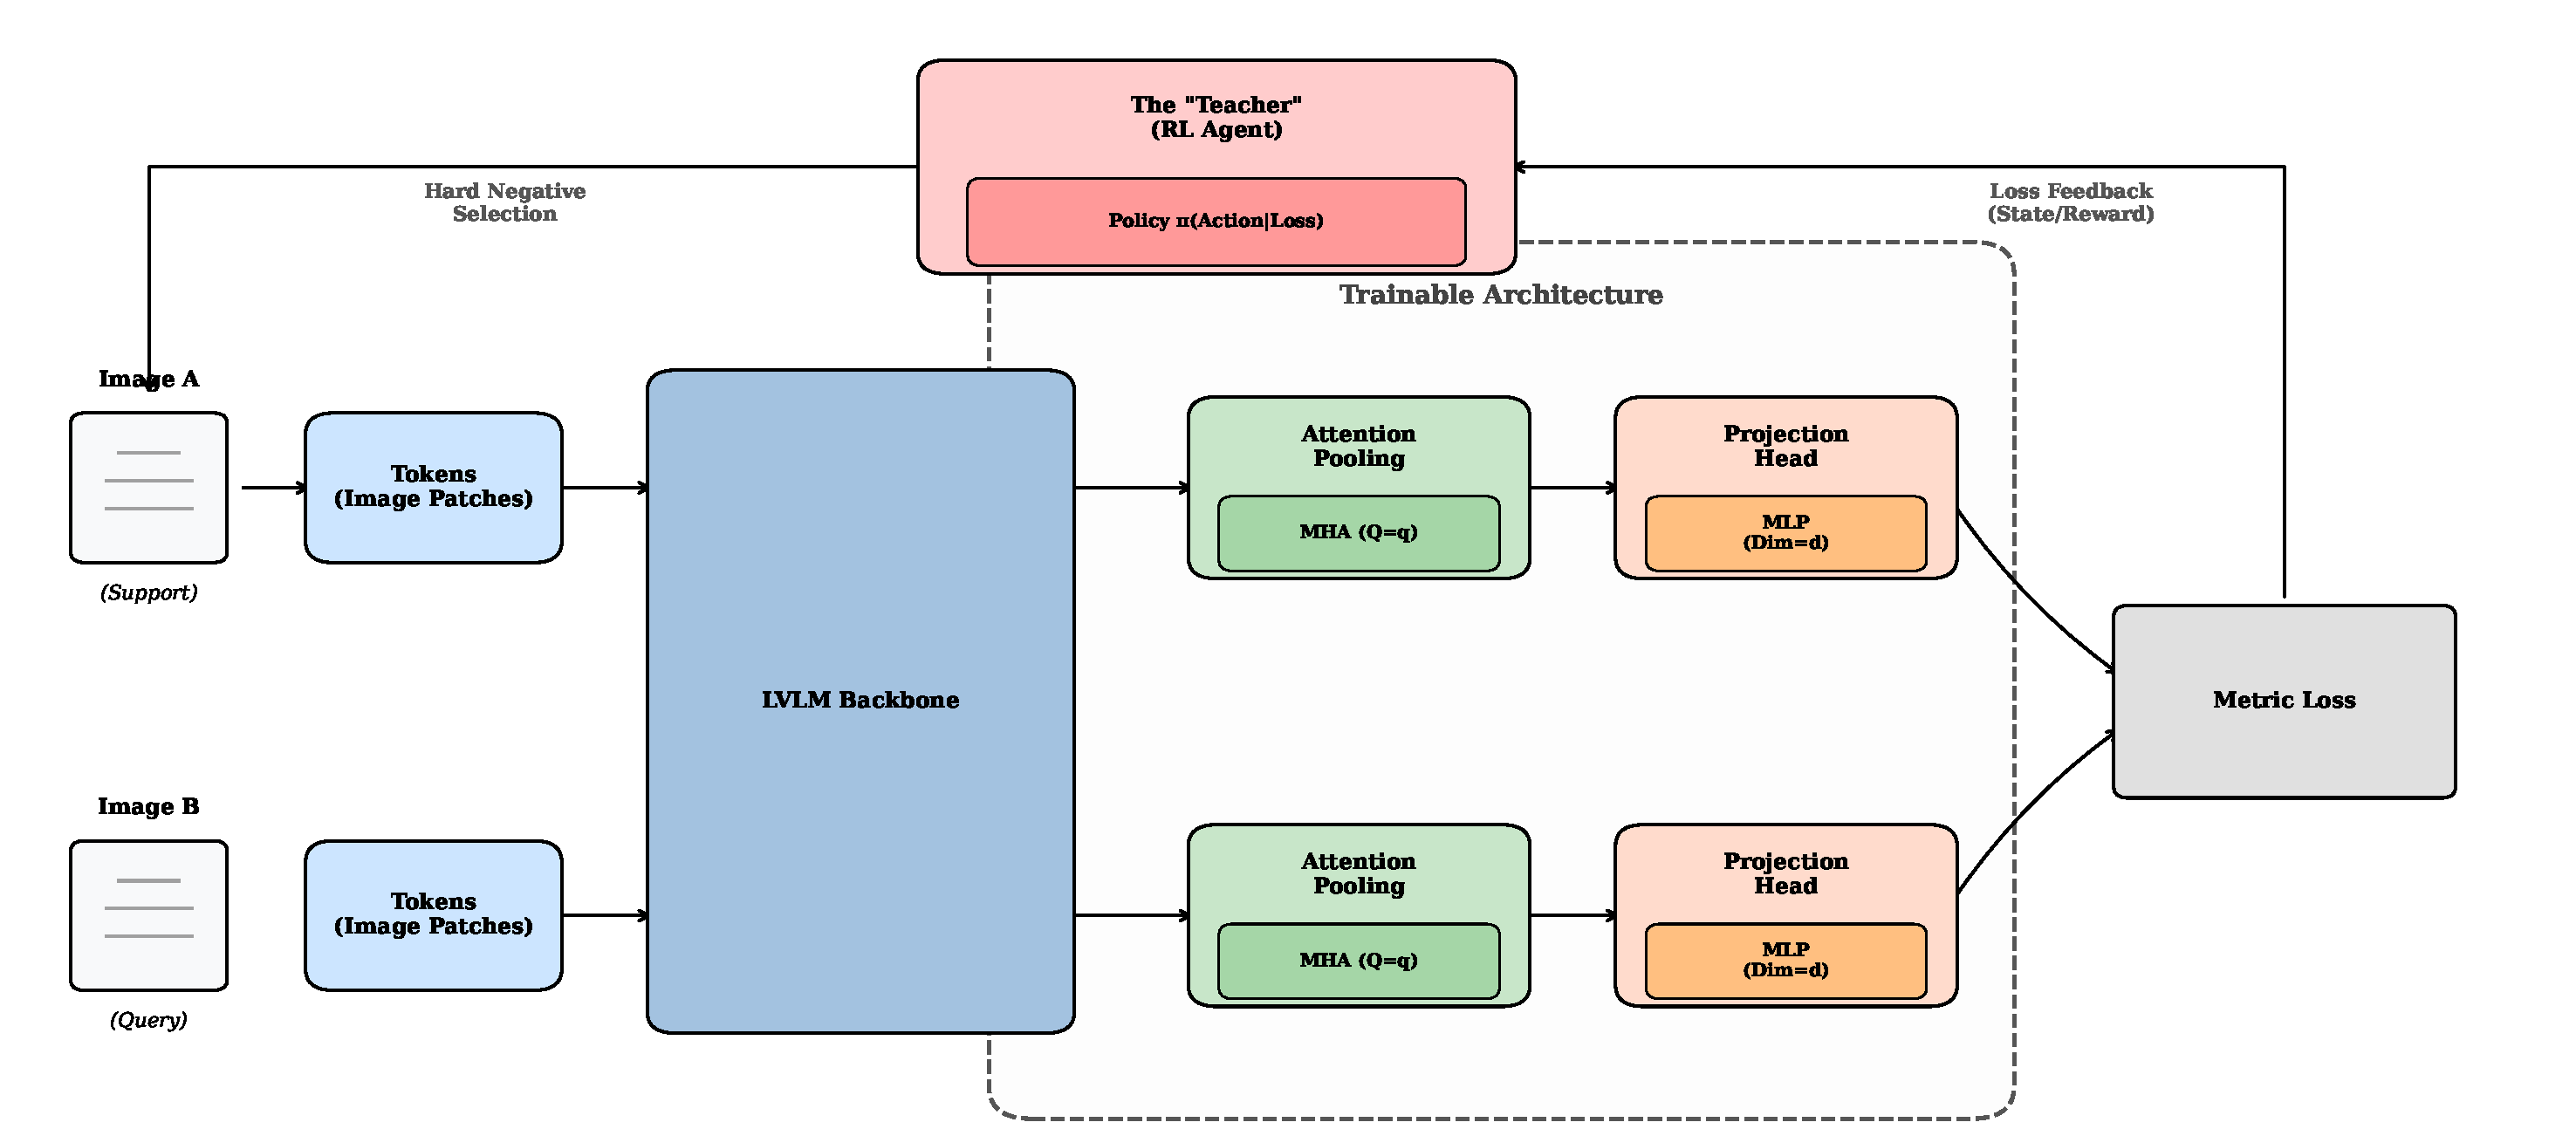
\includegraphics[width=\linewidth, height=0.62\textheight, keepaspectratio]{architecture_with_teacher.pdf}
    \caption{\small Frozen LVLM backbone (InternVL3-2B), conditioned on a rich
      descriptive prompt $\mathcal{P}_r$ $\to$ pooling head (Cross-Modal or Mean/MQAP)
      $\to$ Residual Projection $\to$ Sub-Center CosFace (angular margin).
      An RL \textit{Teacher} agent actively mines \textit{hard negatives} in a curriculum phase.}
  \end{figure}
\end{frame}

% ── SLIDE 6: EMBEDDING STRUCTURE BEFORE TRAINING (Fig. 3a) ───
\begin{frame}{What the Frozen Backbone Already Knows}

  \begin{columns}[T]
    \begin{column}{0.42\linewidth}
      \footnotesize
      Even \textbf{before any training}, the frozen backbone's output layer
      already encodes class-discriminative spatial structure:
      \begin{itemize}\setlength\itemsep{3pt}
        \item Letters concentrate activation at the heading
        \item Invoices spread activation across the tabular body
        \item This pattern is \textbf{prompt-invariant} --- driven purely by visual content
      \end{itemize}
      \vspace{4pt}
      Quantitatively, mean-pooled cosine similarity improves from
      \textbf{7.62\% EER} (input layer) to \textbf{4.78\%} (output layer)
      from backbone contextualization alone.
      \vspace{4pt}
      \textbf{\color{unbblue}But} visually similar classes remain entangled
      without an explicit separation objective $\to$ this motivates the
      \textbf{metric learning loss} (next).
    \end{column}

    \begin{column}{0.56\linewidth}
      \begin{figure}
        \centering
        \includegraphics[width=\linewidth, height=0.56\textheight, keepaspectratio]{prompt_conditioning_visual.pdf}
        \caption{\scriptsize Visual activation per spatial patch at the backbone's
          output layer (base model, no metric learning), for two example documents.
          Letters (left) vs.\ invoices (right) show distinct, class-specific
          spatial signatures --- this is the representation the loss functions
          (next) are trained to sharpen.}
      \end{figure}
    \end{column}
  \end{columns}
\end{frame}

% ── SLIDE 7: LOSSES & GEOMETRY ────────────────────────────────
\begin{frame}{Loss Functions: from Distance to Angular Margin}
  \vfill
  \begin{figure}
    \centering
    \includegraphics[width=\linewidth, keepaspectratio]{losses_embedding_space_wide.pdf}
  \end{figure}
  \vspace{10pt}
  {\footnotesize \textbf{Contrastive/Triplet}: no global geometric anchor, clusters form
  at arbitrary positions and scales. \quad \textbf{ArcFace/CosFace}: hypersphere
  with angular margin --- class-agnostic geometry, transferable to unseen classes.}
  \vspace{8pt}

  {\footnotesize Both ArcFace and CosFace are extended with \textbf{Sub-Center}
  ($k{=}3$ sub-prototypes per class) to handle multi-modal intra-class variance.
  \textit{Circle Loss} was also evaluated but eliminated (high variance in fine search).}
  \vfill
\end{frame}

% ── SLIDE 8: TRAINING PROTOCOL & HYPERPARAMETER SEARCH ───────
\begin{frame}{Training Protocol \& Hyperparameter Search}

  \begin{columns}[T]
    \begin{column}{0.50\linewidth}
      \begin{block}{Three Phases (Bayesian Sweeps)}
        \footnotesize
        \begin{enumerate}\setlength\itemsep{5pt}
          \item \textbf{Coarse} --- 173 runs; two-gate filter
                (5\% EER ceiling $+$ divergence check); \textbf{68.8\%} pass rate
          \item \textbf{Fine} --- 96 runs across 10 groups; LR range
                narrowed to $2$--$10\times10^{-5}$
          \item \textbf{Full Evaluation} --- champion config trained with
                full epochs across all 5 CV splits
        \end{enumerate}
      \end{block}
    \end{column}

    \begin{column}{0.46\linewidth}
      \begin{alertblock}{Key Findings}
        \footnotesize
        \begin{itemize}\setlength\itemsep{4pt}
          \item \textbf{LR} is the dominant hyperparameter across all groups
                ($|r| > 0.87$ with $\log(\text{lr})$)
          \item Margin: Sub-Center CosFace $k{=}3$ converges at $m\approx0.18$--$0.35$;
                ArcFace $k{=}3$ best at $m\approx0.31$
          \item Scale $s = 32$ stable across families
          \item \textit{Circle Loss} did not advance (high variance in fine search)
        \end{itemize}
      \end{alertblock}
      \vspace{4pt}
      {\footnotesize AdamW, \texttt{ReduceLROnPlateau}. Single GPU:
      RTX~4060~Ti (16\,GB) / RTX~4090.}
    \end{column}
  \end{columns}
\end{frame}

% ── SLIDE 9: ABLATION — LOSSES AND TEACHER AGENT ─────────────
\begin{frame}{Ablation: Loss Functions \& \textit{Teacher} Agent}
  \begin{figure}
    \centering
    \includegraphics[width=0.92\linewidth, trim={6em 0 2em 0}, clip, height=0.44\textheight, keepaspectratio]{ablation_heatmap_v2.pdf}
    \caption{\scriptsize Cumulative best EER (across 15 epochs, Phases 1+2) per loss and split
      on LA-CDIP. \textbf{Sub-Center CosFace} achieves the best mean with hard-negative mining (0.95\%).}
  \end{figure}

  \vspace{2pt}
  \centering
  \scriptsize
  \setlength{\tabcolsep}{5pt}
  \renewcommand{\arraystretch}{1.15}
  \begin{tabular}{lccc}
    \toprule
    \textbf{Loss} & \textbf{With Mining} & \textbf{Without Mining} & \textbf{$\Delta$ (pp)} \\
    \midrule
    \cellcolor{winrow}\textbf{Sub-Center CosFace} & \cellcolor{winrow}\textbf{0.95\%} & \cellcolor{winrow}1.22\% & \cellcolor{winrow}$+$0.27 \\
    Sub-Center ArcFace & \textbf{1.15\%} & 1.18\% & $+$0.03 \\
    Triplet            & 1.55\%          & \textbf{1.48\%} & $-$0.07 \\
    Contrastive        & \textbf{2.05\%} & 2.10\% & $+$0.05 \\
    \bottomrule
  \end{tabular}
\end{frame}

% ── SLIDE 9a: POOLING & PROMPT CONDITIONING (DESIGN, Fig. 3b) ─
\begin{frame}{Pooling Architectures \& Prompt Conditioning}

  \begin{columns}[T]
    \begin{column}{0.42\linewidth}
      \footnotesize
      \textbf{Three aggregation strategies} for the backbone's multimodal tokens:
      \begin{itemize}\setlength\itemsep{3pt}
        \item \textbf{Mean Pooling} --- uniform average of all tokens
        \item \textbf{MQAP} --- learned query, attention over the full sequence
        \item \textbf{Cross-Modal} --- two independent queries (visual $+$ text), learned fusion
      \end{itemize}
      \vspace{4pt}
      \textbf{Prompt conditioning:} the backbone is frozen, but the \textit{prompt}
      redirects cross-attention across all 36 layers --- no weight is updated.
      \begin{itemize}\setlength\itemsep{2pt}
        \item $\mathcal{P}_0$: 4 tokens (minimal instruction)
        \item $\mathcal{P}_r$: 77 tokens ($19\times$ longer, layout-focused)
      \end{itemize}
    \end{column}

    \begin{column}{0.56\linewidth}
      \begin{figure}
        \centering
        \includegraphics[width=\linewidth, height=0.56\textheight, keepaspectratio]{prompt_conditioning_attention.pdf}
        \caption{\scriptsize Mean text-to-visual attention at the backbone's output layer
          ($\mathcal{P}_0$ vs.\ $\mathcal{P}_r$, two example documents). $\mathcal{P}_0$ produces a
          diffuse distribution; $\mathcal{P}_r$ concentrates attention on layout-discriminative
          regions, with \emph{no change to any backbone weight}.}
      \end{figure}
    \end{column}
  \end{columns}

  \vspace{2pt}
  {\footnotesize\color{black!50} Quantitative ablation of pooler $\times$ prompt combinations follows next.}
\end{frame}

% ── SLIDE 9b: ABLATION — POOLING & PROMPT CONDITIONING ───────
\begin{frame}{Ablation: Pooling Architecture \& Prompt Conditioning}

  \begin{columns}[T]
    \begin{column}{0.40\linewidth}
      \footnotesize
      Best loss (Sub-Center CosFace $+$ \textit{Teacher}) carried forward to
      compare the three poolers under $\mathcal{P}_0$ and $\mathcal{P}_r$.
      \vspace{4pt}
      \begin{itemize}\setlength\itemsep{4pt}
        \item $\mathcal{P}_r$ improves \textbf{every} pooler, without exception
        \item \textbf{Mean Pool $+\,\mathcal{P}_r$}: best average EER
              (\textbf{0.63\%} $\pm$ 0.48\,pp)
        \item \textbf{Cross-Modal $+\,\mathcal{P}_r$}: 0.91\% $\pm$ 1.10\,pp,
              wins on 4/5 individual splits
        \item MQAP $+\,\mathcal{P}_r$: 0.85\% $\pm$ 0.55\,pp
      \end{itemize}
    \end{column}

    \begin{column}{0.58\linewidth}
      \begin{figure}
        \centering
        \includegraphics[width=\linewidth, height=0.56\textheight, keepaspectratio]{pooler_prompt_ablation.pdf}
        \caption{\scriptsize Cumulative EER (LA-CDIP, 5 splits) per pooler $\times$ prompt
          (Sub-Center CosFace). $\mathcal{P}_r$ improves every pooler.}
      \end{figure}
    \end{column}
  \end{columns}
\end{frame}

% ── SLIDE 10: SOTA COMPARISON ─────────────────────────────────
\begin{frame}{Comparison with the State of the Art --- LA-CDIP}
  \begin{columns}[T]
    \begin{column}{0.44\linewidth}
      \begin{figure}
        \includegraphics[width=\linewidth, height=0.58\textheight, keepaspectratio]{perf_vs_params.pdf}
        \caption{\scriptsize EER vs.\ active parameters (log--log). ArcDoc (star) operates
          $6\times$ below the scaling trend of zero-shot VLMs.}
      \end{figure}
    \end{column}
    \begin{column}{0.54\linewidth}
      \centering
      \scriptsize
      \setlength{\tabcolsep}{3pt}
      \renewcommand{\arraystretch}{1.05}
      \begin{tabular}{llcc}
        \toprule
        \textbf{Category} & \textbf{Method} & \textbf{Params} & \textbf{EER (\%)} \\
        \midrule
        \multirow{2}{*}{\cellcolor{winrow}\textbf{Ours}}
          & \cellcolor{winrow}\textbf{ArcDoc}$_{\text{mean},\mathcal{P}_r}$  & \cellcolor{winrow}2B & \cellcolor{winrow}\textbf{0.63} \\
          & \cellcolor{winrow}\textbf{ArcDoc}$_{\text{cross},\mathcal{P}_r}$ & \cellcolor{winrow}2B & \cellcolor{winrow}\textbf{0.91} \\
        \midrule
        \multirow{5}{*}{Zero-Shot VLM}
          & Qwen3-VL-8B    & 8B  & 1.12 \\
          & InternVL3-14B  & 14B & 1.30 \\
          & InternVL3-8B   & 8B  & 2.13 \\
          & Qwen3-VL-4B    & 4B  & 2.67 \\
          & InternVL3-2B   & 2B  & 29.99 \\
        \midrule
        \multirow{1}{*}{\cellcolor{finerow}Embedding}
          & \cellcolor{finerow}Jina-v4 (base)      & \cellcolor{finerow}4B & \cellcolor{finerow}3.08 \\
        \multirow{1}{*}{\cellcolor{finerow}Fine-tuned}
          & \cellcolor{finerow}Jina-v4 (LoRA $r{=}48$) & \cellcolor{finerow}4B & \cellcolor{finerow}2.23 \\
        \midrule
        \cellcolor{coarserow}Pixel & \cellcolor{coarserow}L2 / Cosine & \cellcolor{coarserow}--- & \cellcolor{coarserow}31.2 / 32.3 \\
        \bottomrule
      \end{tabular}
    \end{column}
  \end{columns}

  \vspace{6pt}
  \begin{block}{}
    \footnotesize
    \textbf{InternVL3-2B zero-shot} (same backbone, no training): 29.99\% EER.
    \textbf{ArcDoc} (same backbone): 0.63\% EER. A $\sim$\textbf{48$\times$} gap
    attributable exclusively to the ArcDoc angular margin head.
  \end{block}
\end{frame}

% ── SLIDE 11: ONGOING WORK — PRODUCTION MODEL / AUGMENTATION ─
\begin{frame}{Ongoing Work: Production Model Training --- Split~3}

  \begin{columns}[T]

    %% ── Left column: configuration ─────────────────────────
    \begin{column}{0.42\linewidth}
      \begin{block}{Configuration}
        \footnotesize
        \begin{itemize}\setlength\itemsep{2pt}
          \item Loss: \textbf{Sub-Center CosFace} ($k{=}3$) $+$ \textit{Teacher}
          \item \textbf{1,748} original training images
          \item \textbf{6} variants per image
          \item \textbf{10,488} augmented images
          \item 120 training classes / 24 \textit{novel}
        \end{itemize}
      \end{block}
      \vspace{4pt}
      \begin{alertblock}{Destination}
        \footnotesize
        Definitive model for publication on the
        \textbf{Hugging Face Hub}.
      \end{alertblock}
      \vspace{4pt}
      {\tiny\textbf{11 operations:}
      Rotation, Perspective, Brightness/Contrast, Blur, Sharpening,
      Gaussian Noise, JPEG Q30--70, Resolution~↓, Crop/Padding,
      Yellowing, Salt\,\&\,Pepper.}
    \end{column}

    %% ── Right column: visual examples ──────────────────────
    \begin{column}{0.56\linewidth}
      \begin{figure}
        \centering
        \includegraphics[width=\linewidth, height=0.48\textheight, keepaspectratio]{augmentation_grid.pdf}
        \caption{\scriptsize Four of the 11 operations (original → result). Training combines 6 at random per image.}
      \end{figure}
      {\tiny\color{black!50} Deployment-oriented pipeline, independent of the paper's
      evaluation protocol and splits.}
    \end{column}

  \end{columns}
\end{frame}

% ── SLIDE 12: ROADMAP ─────────────────────────────────────────
\begin{frame}{Project Roadmap}
\hyphenpenalty=10000\exhyphenpenalty=10000

\vspace{0.4cm}
\begin{center}
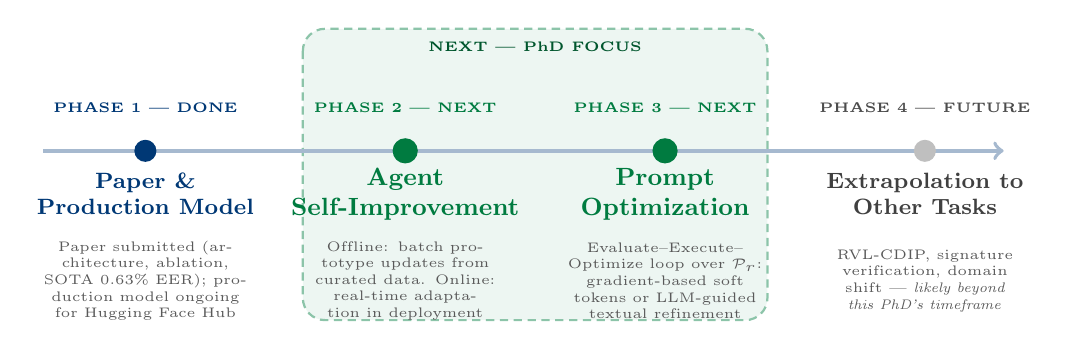
\begin{tikzpicture}[every node/.style={align=center}]

  % ── Highlight band behind Phases 2–3 (PhD focus, next) ───────
  \fill[unbgreen!7, rounded corners=8pt] (3.0,1.55) rectangle (8.9,-2.15);
  \draw[unbgreen!45, densely dashed, line width=0.8pt, rounded corners=8pt]
    (3.0,1.55) rectangle (8.9,-2.15);
  \node[font=\tiny\bfseries, text=unbgreen!70!black] at (5.95,1.32) {NEXT --- PhD FOCUS};

  % ── Baseline arrow ────────────────────────────────────────────
  \draw[->, line width=1.4pt, unbblue!35] (-0.3,0) -- (11.9,0);

  % ── Phase 1: Paper + Production Model (Done / Ongoing) ───────
  \fill[unbblue] (1.0,0) circle (0.14);
  \node[font=\tiny\bfseries, text=unbblue] at (1.0,0.55) {PHASE 1 --- DONE};
  \node[font=\footnotesize\bfseries, text=unbblue] at (1.0,-0.55) {Paper \&\\Production Model};
  \node[font=\tiny, text=black!65, text width=2.6cm] at (1.0,-1.65)
    {Paper submitted (architecture, ablation, SOTA 0.63\% EER); production model ongoing for Hugging Face Hub};

  % ── Phase 2: Agent Self-Improvement (Next, PhD focus) ─────────
  \fill[unbgreen] (4.3,0) circle (0.16);
  \node[font=\tiny\bfseries, text=unbgreen] at (4.3,0.55) {PHASE 2 --- NEXT};
  \node[font=\small\bfseries, text=unbgreen] at (4.3,-0.55) {Agent\\Self-Improvement};
  \node[font=\tiny, text=black!65, text width=2.5cm] at (4.3,-1.65)
    {Offline: batch prototype updates from curated data. Online: real-time adaptation in deployment};

  % ── Phase 3: Prompt Optimization (Next, PhD focus) ────────────
  \fill[unbgreen] (7.6,0) circle (0.16);
  \node[font=\tiny\bfseries, text=unbgreen] at (7.6,0.55) {PHASE 3 --- NEXT};
  \node[font=\small\bfseries, text=unbgreen] at (7.6,-0.55) {Prompt\\Optimization};
  \node[font=\tiny, text=black!65, text width=2.5cm] at (7.6,-1.65)
    {Evaluate--Execute--Optimize loop over $\mathcal{P}_r$: gradient-based soft tokens or LLM-guided textual refinement};

  % ── Phase 4: Extrapolation to Other Tasks (Future, beyond PhD) ─
  \fill[gray!50] (10.9,0) circle (0.14);
  \node[font=\tiny\bfseries, text=gray!60!black] at (10.9,0.55) {PHASE 4 --- FUTURE};
  \node[font=\footnotesize\bfseries, text=gray!50!black] at (10.9,-0.55) {Extrapolation to\\Other Tasks};
  \node[font=\tiny, text=black!65, text width=2.5cm] at (10.9,-1.65)
    {RVL-CDIP, signature verification, domain shift --- \textit{likely beyond this PhD's timeframe}};

\end{tikzpicture}
\end{center}

\vspace{4pt}
{\footnotesize\color{black!55}
\textbf{Phase 1} (done): paper submitted, production model in progress.
\textbf{Phases 2--3} (next, this PhD's focus): agent self-improvement,
then prompt optimization. \textbf{Phase 4} (future): extrapolation to other
document tasks --- likely beyond this PhD's timeline.}

\vspace{2pt}
{\tiny\color{black!45} Phase terminology: Liu et al., \textit{Advances and
Challenges in Foundation Agents}, arXiv:2504.01990 (2025) --- Ch.\,11
(\textit{Online and Offline Agent Self-Improvement}), Sec.\,9.2/Def.\,9
(\textit{Prompt Optimization}).}

\end{frame}

% ── SLIDE 13: THANK YOU ───────────────────────────────────────
\begin{frame}{Thank You}
  \begin{center}
    \vspace{12pt}
    {\Large\bfseries\color{unbblue} Thank You}\\[8pt]
    {\normalsize Questions and discussion}\\[20pt]
    \footnotesize
    \begin{tabular}{rl}
      \textbf{Author:}  & Joao Paulo Costa \\
      \textbf{Advisor:} & Prof.\,Dr.\,Li Weigang \\
      \textbf{Program:} & PPGI / CIC / UnB \\
      \textbf{Contact:} & \texttt{jpcosta1990@gmail.com} \\
    \end{tabular}
  \end{center}
\end{frame}

\end{document}
